\begin{problem}[17]
讨论两端固定的梁在分布载荷作用下的挠度.
\end{problem}
% --------------------------------------------------------------------
\begin{solution}
\begin{minipage}[c]{0.7\linewidth}
该问题的控制参数有: 梁的长度$l$, 梁的抗弯刚度$EI$($E$为杨氏模量, $I$为截面矩), 分布载荷$q(x)$(由特征分布载荷$q_m$和表示分布特征的长度$l_q$来表征), 于是挠度应该是坐标$x$和上述参数的函数:
\[
w = f(x; l; EI; q_m, l_q)
\]
\end{minipage}
\begin{minipage}[c]{0.3\linewidth}
\begin{center}
\usetikzlibrary{calc,intersections,through,backgrounds}
\usetikzlibrary{decorations.pathreplacing,decorations.pathmorphing,arrows}
\usetikzlibrary{shapes}
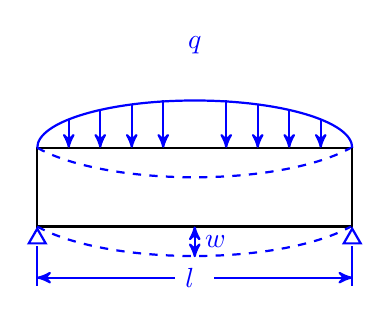
\begin{tikzpicture}
\draw [thick] (-2,-0.5) rectangle (2,0.5);
\draw [thick,blue] (2,0.5) arc (0:180:2 and 0.6) node[midway,above=13pt]{$q$};
\draw[thick,blue,->,>=stealth'] (0.4,1.1)--(0.4,0.5);
\draw[thick,blue,->,>=stealth'] (-0.4,1.1)--(-0.4,0.5);
\draw[thick,blue,->,>=stealth'] (0.8,1.05)--(0.8,0.5);
\draw[thick,blue,->,>=stealth'] (-0.8,1.05)--(-0.8,0.5);
\draw[thick,blue,->,>=stealth'] (1.2,0.98)--(1.2,0.5);
\draw[thick,blue,->,>=stealth'] (-1.2,0.98)--(-1.2,0.5);
\draw[thick,blue,->,>=stealth'] (1.6,0.85)--(1.6,0.5);
\draw[thick,blue,->,>=stealth'] (-1.6,0.85)--(-1.6,0.5);

\draw [thick,blue,dashed] (-2,0.5) arc (210:330:2.3 and 0.75)
                                                    (-2,-0.5) arc (210:330:2.3 and 0.75);
\draw[thick,blue,<->,>=stealth'] (0,-0.5)--(0,-0.89) node[midway,right]{$w$};

\draw (-2,-0.5) node[below,draw=blue,thick,regular polygon, regular polygon sides=3,  inner sep=1.25]{};
\draw (2,-0.5) node[draw=blue,thick,below,regular polygon, regular polygon sides=3,  inner sep=1.25]{};
\draw[thick,blue,>=stealth'](-2,-0.75)--(-2,-1.25) (2,-0.75)--(2,-1.25); \draw[thick,blue,<-,>=stealth'](-2,-1.15)--(-0.25,-1.15) node[right]{$l$}; \draw[thick,blue,<-,>=stealth'](2,-1.15)--(0.25,-1.15);
\end{tikzpicture}
\end{center}
\end{minipage}\vspace{10pt}
上式中的各物理量的量纲分别为:$[w]=[x]=[l]=[l_q]=L$, $[EI]=FL^2$, $[q_m]=FL^{-1}$. 该问题中含有两个独立量纲, 取$l$和$EI$作为基本量, 且组成单位系统, 于是上式可转化为
\begin{equation}\label{eq:17-wl}
\frac{w}{l} = f\bigg(\frac{x}{l},1,1,\frac{q_m}{EI/l^3},\frac{l_q}{l}\bigg)
= f\bigg(\frac{x}{l},\frac{q_ml^3}{EI},\frac{l_q}{l}\bigg)
\end{equation}
因此, 只要保持
\[
\frac{q_ml^3}{EI}=\mathrm{const},\qquad \frac{l_q}{l}=\mathrm{const}
\]
就会有同一个无量纲挠度分布$w = lf(x/l)$. 对比式(\ref{eq:17-wl})与书本\cite{tan_dimensional_2011}第50页式(4.3)的简支梁的结果, 发现结果在形式上一样的, 但由于这两种情形在物理上并不一样, 可知量纲分析的结果中的$f$函数的形式必然不同.
\end{solution}
\label{problem:17}
